\documentclass[]{book}
\usepackage{lmodern}
\usepackage{amssymb,amsmath}
\usepackage{ifxetex,ifluatex}
\usepackage{fixltx2e} % provides \textsubscript
\ifnum 0\ifxetex 1\fi\ifluatex 1\fi=0 % if pdftex
  \usepackage[T1]{fontenc}
  \usepackage[utf8]{inputenc}
\else % if luatex or xelatex
  \ifxetex
    \usepackage{mathspec}
  \else
    \usepackage{fontspec}
  \fi
  \defaultfontfeatures{Ligatures=TeX,Scale=MatchLowercase}
\fi
% use upquote if available, for straight quotes in verbatim environments
\IfFileExists{upquote.sty}{\usepackage{upquote}}{}
% use microtype if available
\IfFileExists{microtype.sty}{%
\usepackage[]{microtype}
\UseMicrotypeSet[protrusion]{basicmath} % disable protrusion for tt fonts
}{}
\PassOptionsToPackage{hyphens}{url} % url is loaded by hyperref
\usepackage[unicode=true]{hyperref}
\hypersetup{
            pdftitle={ICT Gender-Equality Paradox Re-Analysis},
            pdfauthor={Mandy Davis},
            pdfborder={0 0 0},
            breaklinks=true}
\urlstyle{same}  % don't use monospace font for urls
\usepackage{natbib}
\bibliographystyle{plainnat}
\usepackage{longtable,booktabs}
% Fix footnotes in tables (requires footnote package)
\IfFileExists{footnote.sty}{\usepackage{footnote}\makesavenoteenv{long table}}{}
\usepackage{graphicx,grffile}
\makeatletter
\def\maxwidth{\ifdim\Gin@nat@width>\linewidth\linewidth\else\Gin@nat@width\fi}
\def\maxheight{\ifdim\Gin@nat@height>\textheight\textheight\else\Gin@nat@height\fi}
\makeatother
% Scale images if necessary, so that they will not overflow the page
% margins by default, and it is still possible to overwrite the defaults
% using explicit options in \includegraphics[width, height, ...]{}
\setkeys{Gin}{width=\maxwidth,height=\maxheight,keepaspectratio}
\IfFileExists{parskip.sty}{%
\usepackage{parskip}
}{% else
\setlength{\parindent}{0pt}
\setlength{\parskip}{6pt plus 2pt minus 1pt}
}
\setlength{\emergencystretch}{3em}  % prevent overfull lines
\providecommand{\tightlist}{%
  \setlength{\itemsep}{0pt}\setlength{\parskip}{0pt}}
\setcounter{secnumdepth}{5}
% Redefines (sub)paragraphs to behave more like sections
\ifx\paragraph\undefined\else
\let\oldparagraph\paragraph
\renewcommand{\paragraph}[1]{\oldparagraph{#1}\mbox{}}
\fi
\ifx\subparagraph\undefined\else
\let\oldsubparagraph\subparagraph
\renewcommand{\subparagraph}[1]{\oldsubparagraph{#1}\mbox{}}
\fi

% set default figure placement to htbp
\makeatletter
\def\fps@figure{htbp}
\makeatother

\usepackage{booktabs}
\usepackage{amsthm}
\makeatletter
\def\thm@space@setup{%
  \thm@preskip=8pt plus 2pt minus 4pt
  \thm@postskip=\thm@preskip
}
\makeatother

\title{ICT Gender-Equality Paradox Re-Analysis}
\author{Mandy Davis}
\date{2020-07-26}

\begin{document}
\maketitle

{
\setcounter{tocdepth}{1}
\tableofcontents
}
\chapter{Introduction}\label{introduction}

In 2018, Stoet \& Geary published a paper titled, ``The Gender-Equality
Paradox in Science, Technology, Engineering, and Mathematics
Education.'' This paper was the first to introduce this idea of a
gender-equality paradox in Science, Technology, Engineering, and
Mathematics (STEM) education, and therefore gained traction in the
popular media (e.g., \citet{stoetGenderEqualityParadoxScience2018a}).
The STEM gender-equality paradox (STEM-GEP) represents the
counter-intuitive, negative correlation between gender equality (as
measured by the Global Gender Gap Index (GGGI)) and the percentage of
STEM graduates who are women. That is, countries with higher gender
equality tend to have a lower percentage of STEM graduates who are
women.

These findings are controversial for multiple reasons. First, one can
imagine how the results could used as evidence in support of politicized
ideas about gender differences in the pursuit of STEM: in countries with
higher gender equality, women presumably face fewer barriers to pursuing
a STEM education, thus the low percentage of women STEM graduates could
reflect women's choice to pursue other fields due to intrinsic factors
like interest. Similarly, one might argue that the high percentage of
women STEM graduates in countries with low gender equality reflects a
choice to pursue STEM due to extrinsic factors like financial
incentives.

Secondly, Stoet \& Geary's findings are controversial due to several
errors in the original paper that have since been corrected, though
these changes did not impact the conclusions of the paper. Richardson et
al.'s \citeyearpar{richardsonThereGenderEqualityParadox2020a} commentary
article illuminates two major aspects of Stoet \& Geary's
\citeyearpar{stoetGenderEqualityParadoxScience2018a} STEM-GEP paper that
merit consideration. Richardson et al. (2020) point out that the x-axis
of the STEM-GEP was misidentified. The original paper included a graph
with the x-axis labeled ``Women Among STEM Graduates (\%)'', which has
been corrected to ``Propensity of Women to Graduate With STEM Degrees''
in the updated, 2020 paper. The new label still evokes confusion, as
``propensity'' could be interpreted in various ways. An even more
representative x-axis label would read, ``Women Among STEM Graduates
(\%) When Adjusted for Differences in Graduation Numbers of Men and
Women.'' The x-axis label was changed because the data used in that
correlation were not, in fact, data concerning the percent of women
among STEM graduates. Rather, the data used and what Stoet \& Geary
(2020) now call \emph{propensity}, is an estimate of the percentage of
women among STEM graduates after adjusting for equal graduation rates
among men and women.

Richardson et al. (2020) also bring attention to the importance of which
gender equality index measure is used. When re-analyzing the data with
the Basic Index of Gender Equality (BIGI), the correlation between
percent of women among STEM graduates and gender equality ceases to
exist. However, in a reply to Richardson et al., Stoet \& Geary
\citeyearpar{stoetGenderEqualityParadoxPart2020a} argue that the BIGI
(which they developed themselves) is not an appropriate index to compare
to the STEM gender data, as the BIGI measures merely well-being and not
empowerment. Richardson, who directs the GenderSci Lab at Harvard
University, continues to write about this controversy in a series of
blog posts on the lab's website,
\href{https://www.genderscilab.org/blog/the-gendersci-lab-takes-on-the-gender-equality-paradox-hypothesis-introduction-and-primer}{GenderSci
Lab Blog Series}.

\section{The ICT Gender-Equality
Paradox}\label{the-ict-gender-equality-paradox}

Using Stoet \& Geary's (2018) paper as a launching pad, the UNESCO for
the EQUALS Skills Coalition dedicated part of their 2019 report on
digital skills and gender \citep{westBlushIfCould2019a} to a Thinkpiece
introducing the Information and Communication Technology (ICT) version
of the STEM-GEP, henceforth the ICT-GEP. ICT refers to education
programs that one might conceptualize as technology programs and broadly
refers to computer science and related programs. More specifically,
UNESCO provides a definition\footnote{UNESCO defines ICT education and
  training as ``(1) the study of techniques and acquisition of skills to
  produce newspapers, radio/television programmes, films/videos,
  recorded music and graphic reproduction with ICT; (2) the study of the
  design and development of computer systems and computing environments;
  (3) the study of using computers and computer software and
  applications for different purposes; and (4) the study of planning,
  designing, developing, maintaining and monitoring electronic
  equipment, machinery and systems''} outlining four categories that
qualify as ICT. The ICT-GEP follows the same trend as the STEM-GEP, that
is, the higher the gender equality (GGGI) of a given country, the lower
the percentage of ICT graduates who are women. Though UNESCO's analysis
of the ICT-GEP mostly mirrors that of Stoet \& Geary (2018), the ICT-GEP
has not received criticism and undergone a re-analysis like the STEM-GEP
has.

\section{The Present Research}\label{the-present-research}

The ICT-GEP Thinkpiece lacks many details concerning the method of
analysis; additionally, the ICT-GEP has only been measured using one
correlation strategy. The present research aims to investigate the
ICT-GEP data in order to fill those methodological disclosure gaps, as
well as re-analyze the ICT-GEP using two alternative methods of
correlating ICT data with GGGI data.

Following from the three related, but disparate approaches, the present
research asks, for the ICT-GEP, do the three approaches result in
parallel results?

\chapter{Visualizing the ICT-GEP}\label{maps}

Before diving into the data, these maps offer a visual explanation of
the ICT-GEP when using the analysis method from the UNESCO think piece.

\section{Percent of women among ICT Graduates
worldwide}\label{percent-of-women-among-ict-graduates-worldwide}

\begin{center}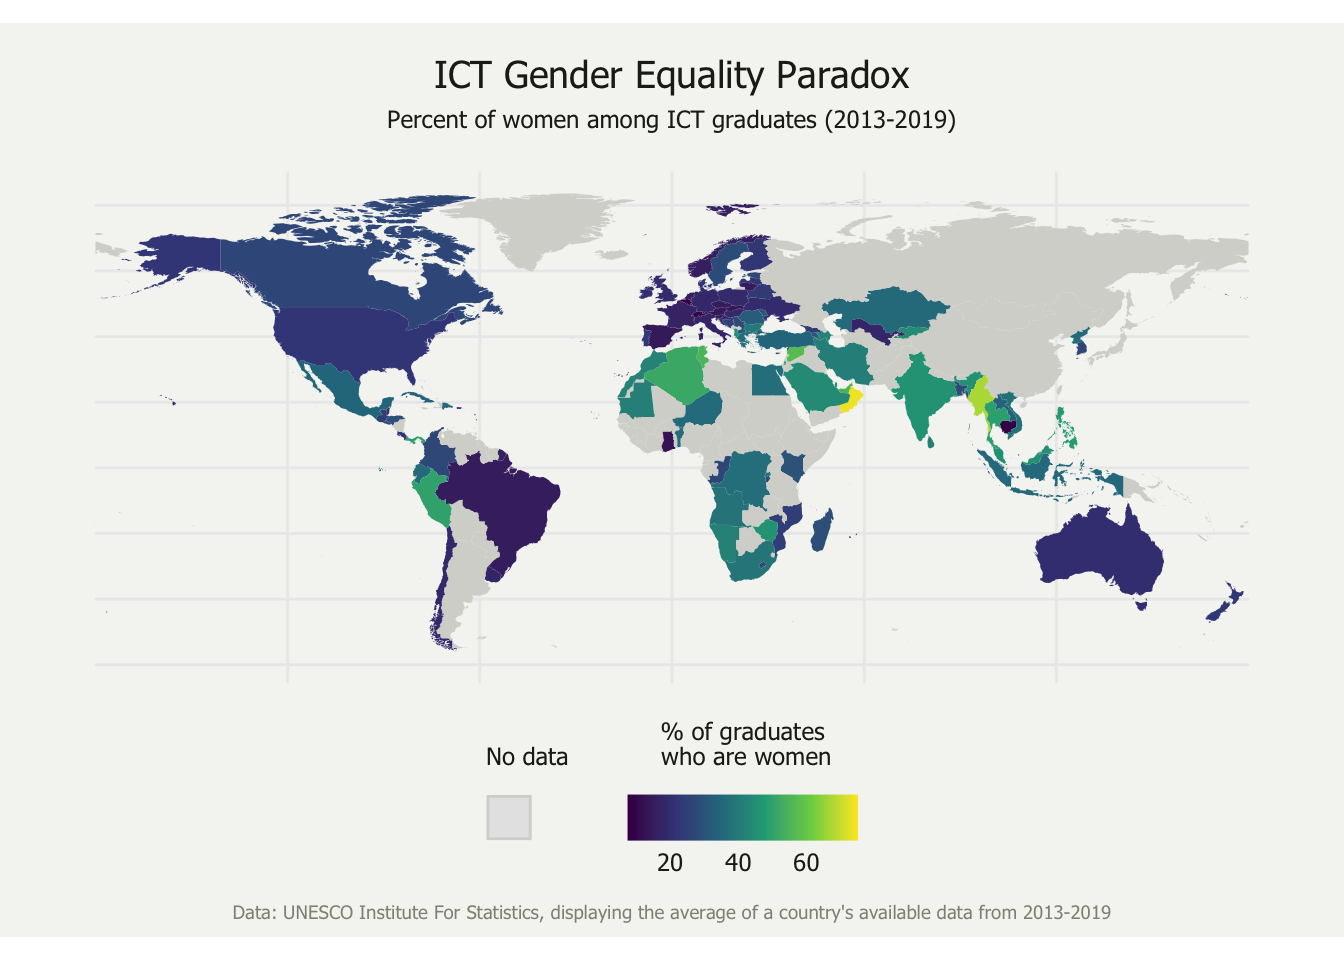
\includegraphics{bookdown-demo_files/figure-latex/ict_map-1} \end{center}

Note the visual reversal of colors when comparing the ICT map to the
GGGI map. This is exactly the idea behind the ICT-GEP: the higher the
gender equality, the lower the percentage of women among ICT graduates.

\section{Global Gender Gap Index
worldwide}\label{global-gender-gap-index-worldwide}

\begin{center}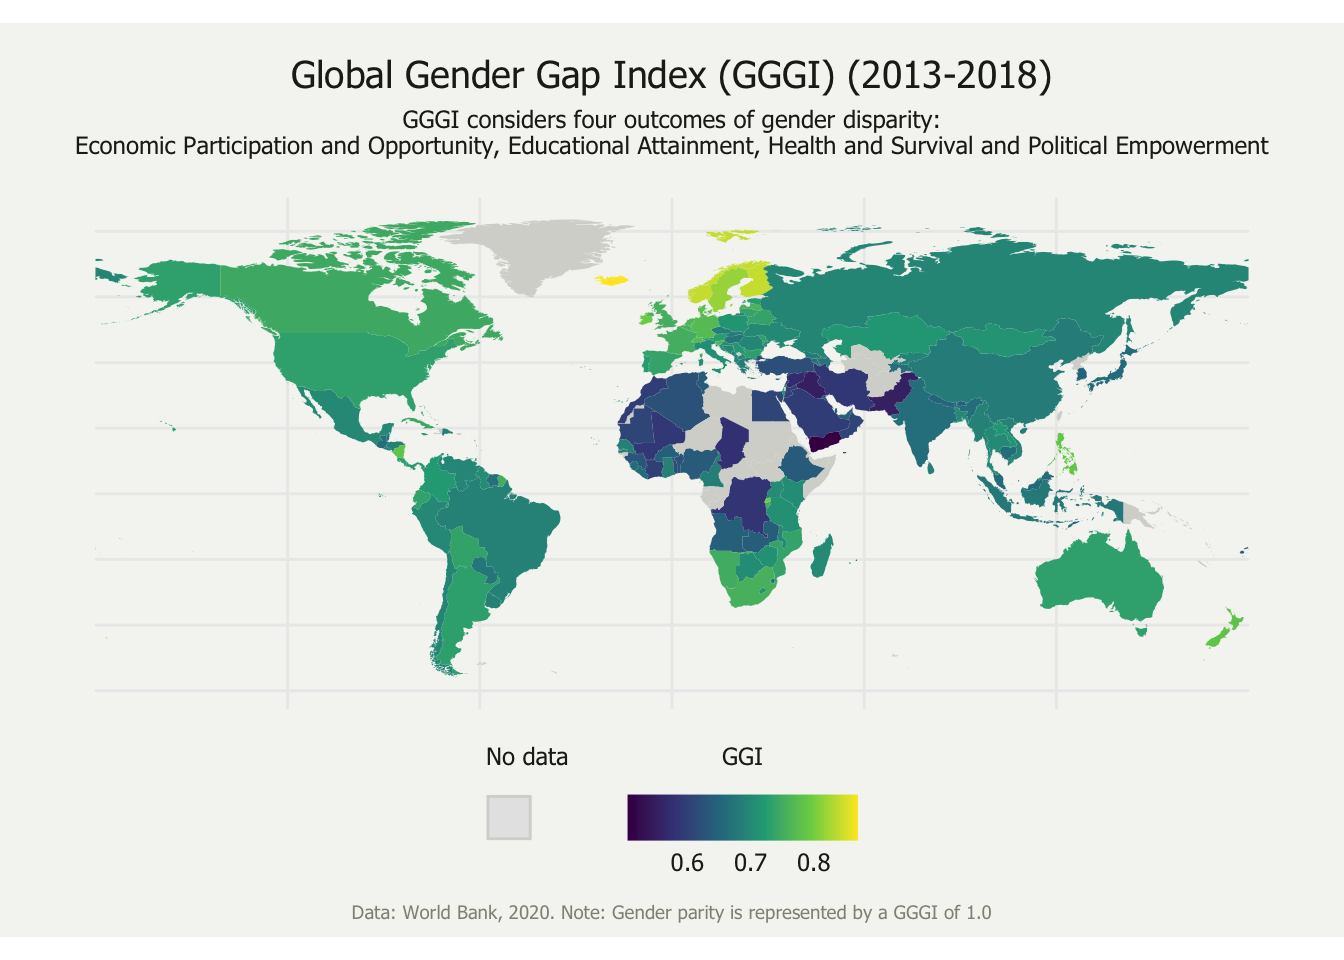
\includegraphics{bookdown-demo_files/figure-latex/ggi_map-1} \end{center}

\chapter{Methods}\label{methods}

\section{Clarifying the UNESCO statistics and their usage in prior
literature}\label{clarifying-the-unesco-statistics-and-their-usage-in-prior-literature}

Both Stoet \& Geary (2018) and the think piece utilize The UNESCO
Institute for Statistics (UIS) education database. Though the two
analyses seemingly mirror each other, a closer look suggests that there
are important nuances in the application of the UIS statistics in both.
To offer clarity, definitions of two important statistics, henceforth
\textbf{percent\_of\_women} and \textbf{percent\_of\_ict}, follows.

\subsection{\texorpdfstring{Percentage of female graduates from ICT
programs in tertiary education:
\textbf{percent\_of\_women}}{Percentage of female graduates from ICT programs in tertiary education: percent\_of\_women}}\label{percentage-of-female-graduates-from-ict-programs-in-tertiary-education-percent_of_women}

This percentage is derived from dividing the number of women who
graduate with an ICT tertiary degree by the number of women who graduate
with any tertiary degree. For example, in Algeria, this number was
2.13\% in 2016, whereas in the US, it was 1.53\% in 2016.

\subsection{\texorpdfstring{Percentage of graduates from ICT programs in
tertiary education who are female:
\textbf{percent\_of\_ict}}{Percentage of graduates from ICT programs in tertiary education who are female: percent\_of\_ict}}\label{percentage-of-graduates-from-ict-programs-in-tertiary-education-who-are-female-percent_of_ict}

This percentage is derived from dividing the number of women who
graduate with an ICT tertiary degree by the total number of men and
women who graduate with an ICT tertiary degree. Note that this statistic
does not account for any gender differences in overall tertiary degrees
earned. Presumably, the number of ICT tertiary degrees earned is
correlated with the total number of degrees earned, so differences in
these base rates should be considered in analyses, contrary to the
arguments of Richardson et al. (2020). As an example of what these
\textbf{percent\_of\_ict} statistics look like, 54.28\% of Algerian ICT
tertiary graduates in 2016 were women, whereas 23.61\% of American ICT
tertiary graduates in 2016 were women.

\subsection{Which statistics do Stoet \& Geary (2018) and the ICT-GEP
think piece
use?}\label{which-statistics-do-stoet-geary-2018-and-the-ict-gep-think-piece-use}

Stoet \& Geary (2018) plug the \textbf{percent\_of\_women} data into a
formula they claim represents the percentage of women in STEM when equal
numbers of men and women enroll at the university. This formula is
\(a/(a+b)\) where \(a\) is the ``percentage of women who graduate with
STEM degrees (relative to all women graduating)'' and \(b\) is ``the
percentage of men who graduate with STEM degrees (relative to all men
graduating)''. Stoet \& Geary's (2020, p.~1). The explanation of this
formula states that ``the resulting number can be interpreted as the
percentage of women in STEM when equal numbers of men and women enroll
at university'' (Stoet \& Geary 2020, p.~1). There are a few notable
subtleties about this language: the UIS education data is collected on
the country level (not the university level) and additionally, the data
the authors utilized represent when equal numbers of men and women
\emph{graduate with tertiary degrees} within that country (there is a
subtle difference between enrollment and completion/graduation). Lastly,
Stoet \& Geary (2018) take the average of each country's available data
from 2012-2015.

Taking a different approach, ICT-GEP think piece utilizes the
\textbf{percent\_of\_ict} data and does not transform this data in any
way. It is unclear what criteria were used for determining which year's
data was selected for the analysis, as there was not a consistent method
for each country's data. The Think piece was published on May 22, 2019
\citep{khazanMoreGenderEquality2018}, which was before the 2018 UNESCO
Education data was released on September 12, 2019
\citep{UISEducationData2019}. However, this does not explain the
inconsistency in year selection. For example, the think piece uses 2017
data for Singapore (latest data available), but 2016 data for
Switzerland though there is 2017 data available. Though the think piece
visually and verbally presents the negative correlation between GGGI and
the percent of women among ICT graduates, the authors do not provide any
further statistical detail (e.g., Pearson's \emph{r}). The language
presented on the think piece correlation plot suggests confusion (or
else, lack of precision) between \textbf{percent\_of\_women} and
\textbf{percent\_of\_ict}. As mentioned, the think piece plots the
``Percentage of graduates from ICT programs in tertiary education who
are female'' (\textbf{percent\_of\_ict}); however, labels on opposite
ends of the graph read, ``HIGH percentage of women completing ICT
programmes'' and ``LOW percentage of women completing ICT programmes.''
This language describes to the \textbf{percent\_of\_women} data, though
that is not what was plotted in the think piece.

\section{The present research}\label{the-present-research-1}

Stoet \& Geary (2018) and the think piece represent two different
methods for understanding the correlation between GGGI and the
percentage of ICT tertiary graduates who are women, the
\textbf{percent\_of\_women} and \textbf{percent\_of\_ict} approaches,
respectively. In line with prior research that is interested in
correlations with the GGGI \citep{zentnerSteppingOutCaveman2012}, a
third method is proposed here. This method, henceforth
\textbf{ict\_disparity}, examines the correlation between the GGGI and
the ICT graduation sex-difference index. All three methods will be
compared using the \texttt{corcor()} function to determine whether each
of the three strategies produce the same correlation. As a summary, the
following three correlations will be computed with the ICT data:

\begin{itemize}
\tightlist
\item
  Method \#1: the \textbf{percent\_of\_ict} approach (UNESCO think
  piece)
\item
  Method \#2: the \textbf{percent\_of\_women} propensity approach (Stoet
  \& Geary)
\item
  Method \#3: the \textbf{ict\_disparity} approach
\end{itemize}

All data is available for free download online
(\href{http://data.uis.unesco.org/Index.aspx?DataSetCode=EDULIT_DS\&popupcustomise=true\&lang=en\#}{ICT
data},
\href{https://tcdata360-backend.worldbank.org/api/v1/datasets/743/dump.csv}{GGGI
data}). For all ICT variables, each country's value was determined by
averaging all available data from 2013-2019. Each country's GGGI value
represents the average GGGI across the years 2013 to 2018 (2019 data not
available). Though 2019 data is included in the ICT data, but not the
GGGI data, only two countries, Georgia and Kazakhstan, have 2019 ICT
data.

\textbf{The exact data files and R script used for this analysis can be
found
\href{https://github.com/mandydavis/ict-gep-re-analysis/tree/master/data-\&-R-script}{here}.
Reproduction is encouraged.}

\chapter{Analysis}\label{analysis}

\section{Variables}\label{variables}

The normality of all six variables needed for the correlations is
examined via Shapiro-Wilk tests for normality:

\begin{enumerate}
\def\labelenumi{\arabic{enumi}.}
\tightlist
\item
  percentage of women graduates who graduate from ICT programs,
\item
  percentage of men graduates who graduate from ICT programs,
\item
  percentage of women among ICT graduates,
\item
  percentage of women among ICT graduates adjusted for the disparity in
  the ratio of women to men who graduate from all programs,
\item
  disparity between the percentage of all women versus all men graduates
  who graduate from an ICT program, and
\item
  GGGI
\end{enumerate}

\section{Normality}\label{normality}

Of these six variables, only three follow a normal distribution:
variable (3) variable (5), and variable (6). The table below displays
all results of the Shapiro-Wilk tests. Because Pearson's correlation
coefficient (\emph{r}) is the metric of interest, no transformations to
the data are needed because Pearson's \emph{r} requires continuous, but
not normal data.

\begin{longtable}[]{@{}lll@{}}
\toprule
variable & W & p-value\tabularnewline
\midrule
\endhead
\textbf{1} & 0.7473 & 5.056e-12\tabularnewline
\textbf{2} & 0.9033 & 1.499e-06\tabularnewline
\textbf{3} & 0.9693 & 0.0170\tabularnewline
\textbf{4} & 0.9498 & 0.0007\tabularnewline
\textbf{5} & 0.9809 & 0.1433\tabularnewline
\textbf{6} & 0.9890 & 0.5647\tabularnewline
\bottomrule
\end{longtable}

\section{Outliers and data omission}\label{outliers-and-data-omission}

Mahalonobis \(D^{2}\) values were computed for four of the six
variables. The other two variables, variables (4) and (5) were omitted,
as they were computed directly using variables (1) and (2). Including
these variables and thus, their dependencies, will not allow for
Mahalonobis \(D^{2}\) calculations to be possible.

The Q-Q plot below displays each of the countries' Mahalonobis \(D^{2}\)
values (the seven countries that deviate the most are labeled with their
iso\_a3 country code).

\begin{center}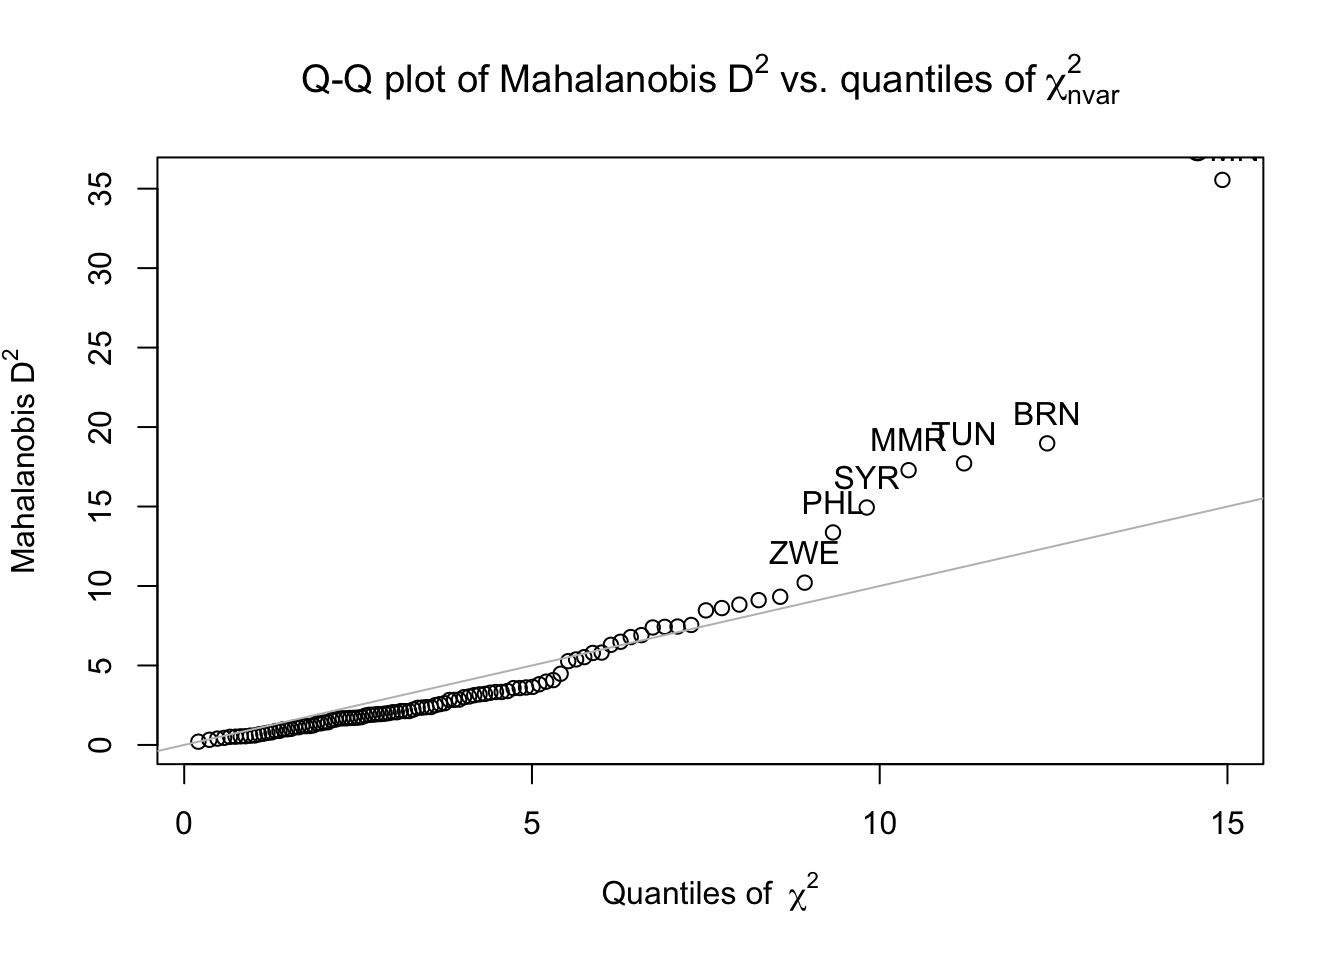
\includegraphics{bookdown-demo_files/figure-latex/normality_outliers-1} \end{center}

The figure below shows bivariate scatter plots, histograms, and the
Pearson correlations for and between each of the four variables, with
any outliers marked with a blue dot. Only one country, Oman (iso\_a3
`OMN'), has a Mahalonobis \(D^{2}\) value of greater than 25. Therefore,
Oman is the sole country to be removed from the analysis for being an
outlier.

\begin{center}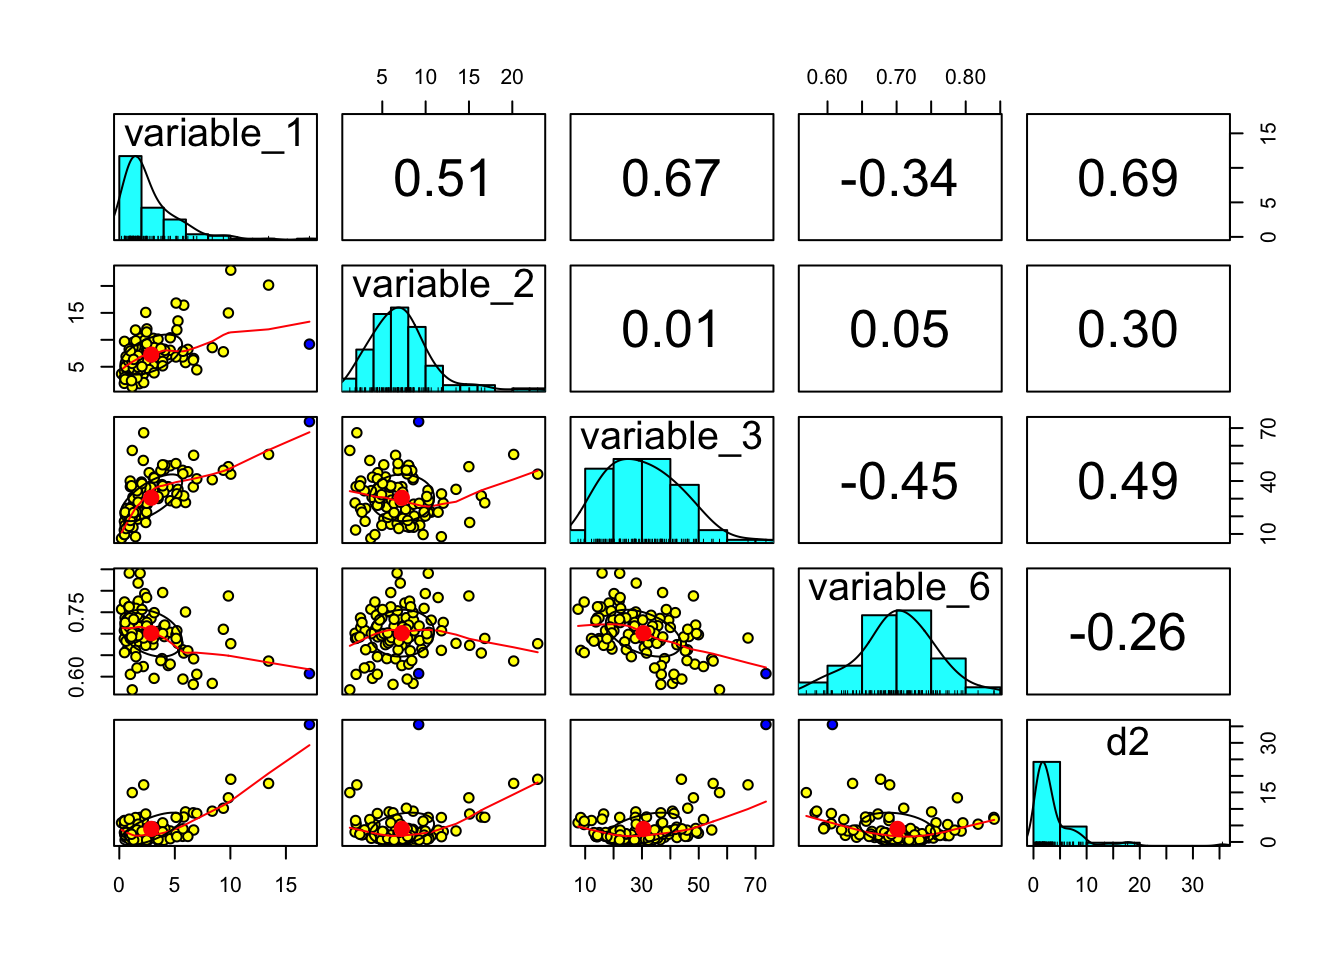
\includegraphics{bookdown-demo_files/figure-latex/outlier_pairs_panels-1} \end{center}

However, in order to correctly compare the three correlations, an
identical set of countries must be the subject of each. The second and
third correlations depend on the existence of data for variables (1) and
(2), whereas the third correlation depends on the existence of data for
variable (3). One country, Sri Lanka, has data for variable (3), but not
variables (1) and (2). Thus, Sri Lanka was the second and final country
to be removed from the analysis. This leaves 102 remaining countries for
which sufficient data is available.

\section{Data description}\label{data-description}

Descriptive statistics for the 102 countries and the bivariate scatter
plots, histograms, and the Pearson correlations for the data after
removing the outlier:

\begin{verbatim}
##            vars   n  mean    sd median trimmed   mad    min   max range  skew kurtosis   se
## variable_1    1 102  2.74  2.41   1.74    2.32  1.20   0.20 13.44 13.24  1.84     3.83 0.24
## variable_2    2 102  7.24  3.74   6.82    6.83  2.72   1.25 22.93 21.68  1.42     3.26 0.37
## variable_3    3 102 30.09 12.60  28.40   29.53 13.52   7.49 67.35 59.86  0.39    -0.48 1.25
## variable_4    4 102 25.94 13.04  23.80   24.93 14.58   4.62 61.17 56.55  0.55    -0.60 1.29
## variable_5    5 102 -4.50  3.10  -4.31   -4.39  3.25 -12.89  2.55 15.44 -0.36    -0.14 0.31
## variable_6    6 102  0.70  0.05   0.70    0.70  0.05   0.57  0.84  0.27 -0.06     0.15 0.01
\end{verbatim}

\begin{center}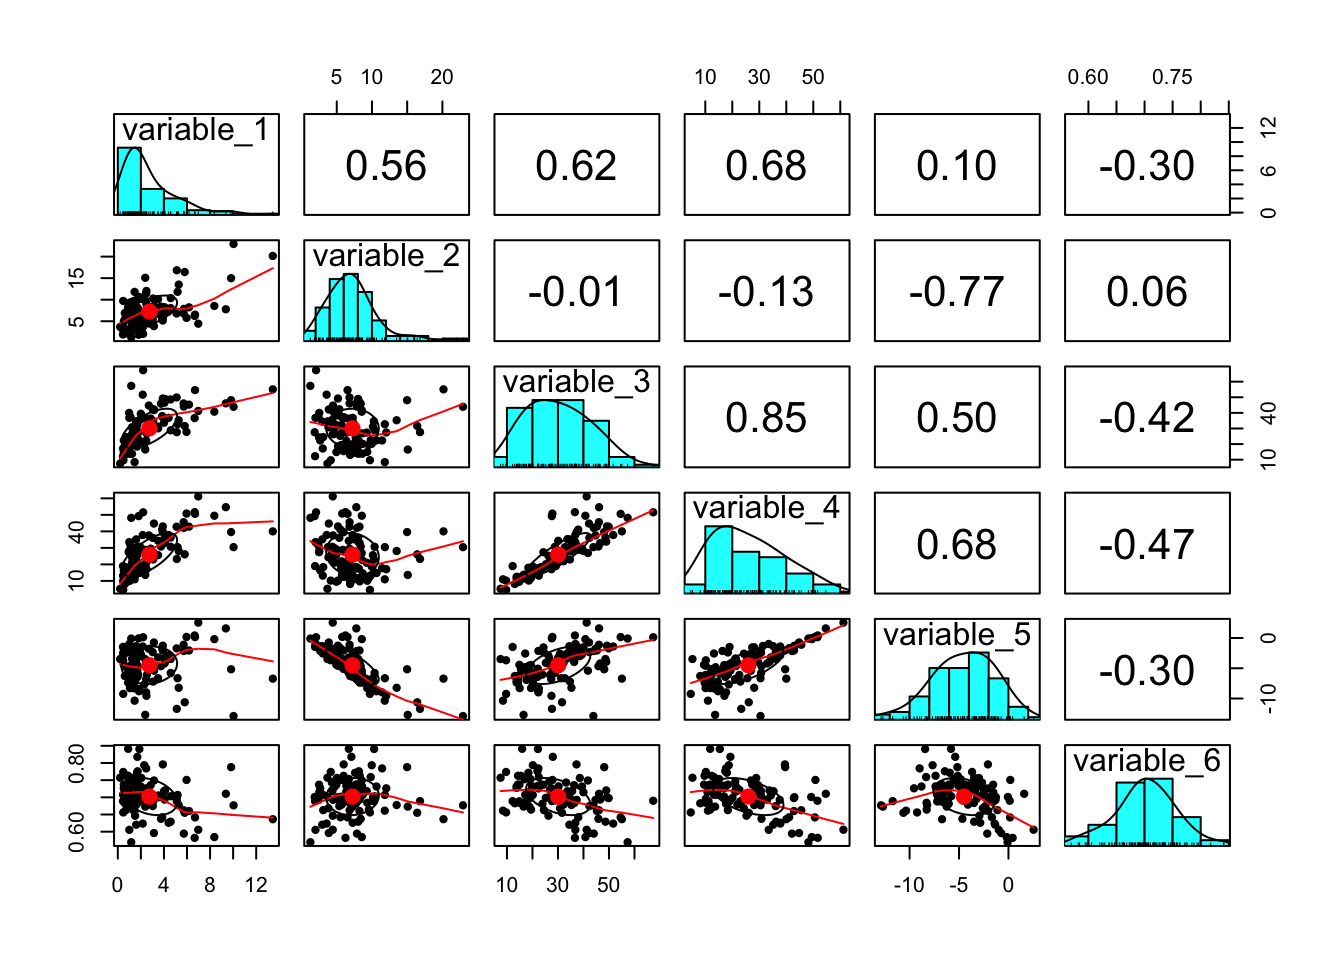
\includegraphics{bookdown-demo_files/figure-latex/description-1} \end{center}

The ICT-GEP Thinkpiece does not offer an explanation regarding the
consideration or removal of outliers. However, through a simple count of
the countries listed in the think piece's reference data, it appears
that only 79 countries were included in the analysis.

\chapter{Results}\label{results}

\section{\texorpdfstring{The ICT-GEP using \textbf{percent\_of\_ict}
data (correlation method
\#1)}{The ICT-GEP using percent\_of\_ict data (correlation method \#1)}}\label{the-ict-gep-using-percent_of_ict-data-correlation-method-1}

After an investigation of the data used in the UNESCO Thinkpiece, this
method exactly replicates the method employed there given the available
information. For example, this analysis examines 102 countries, whereas
the Thinkpiece appears to examine 79. Because the method for selecting
those 79 countries is unknown, that aspect is not replicated. The
Thinkpiece also provides no inferential statistics regarding the
correlation depicted in the ICT-GEP plot. Using the same correlation
method, but 102 country's data, the GGGI and the percent of women among
ICT graduates are moderately, negatively correlated (\emph{r} = -0.43,
\emph{p} \textless{} 0.001).

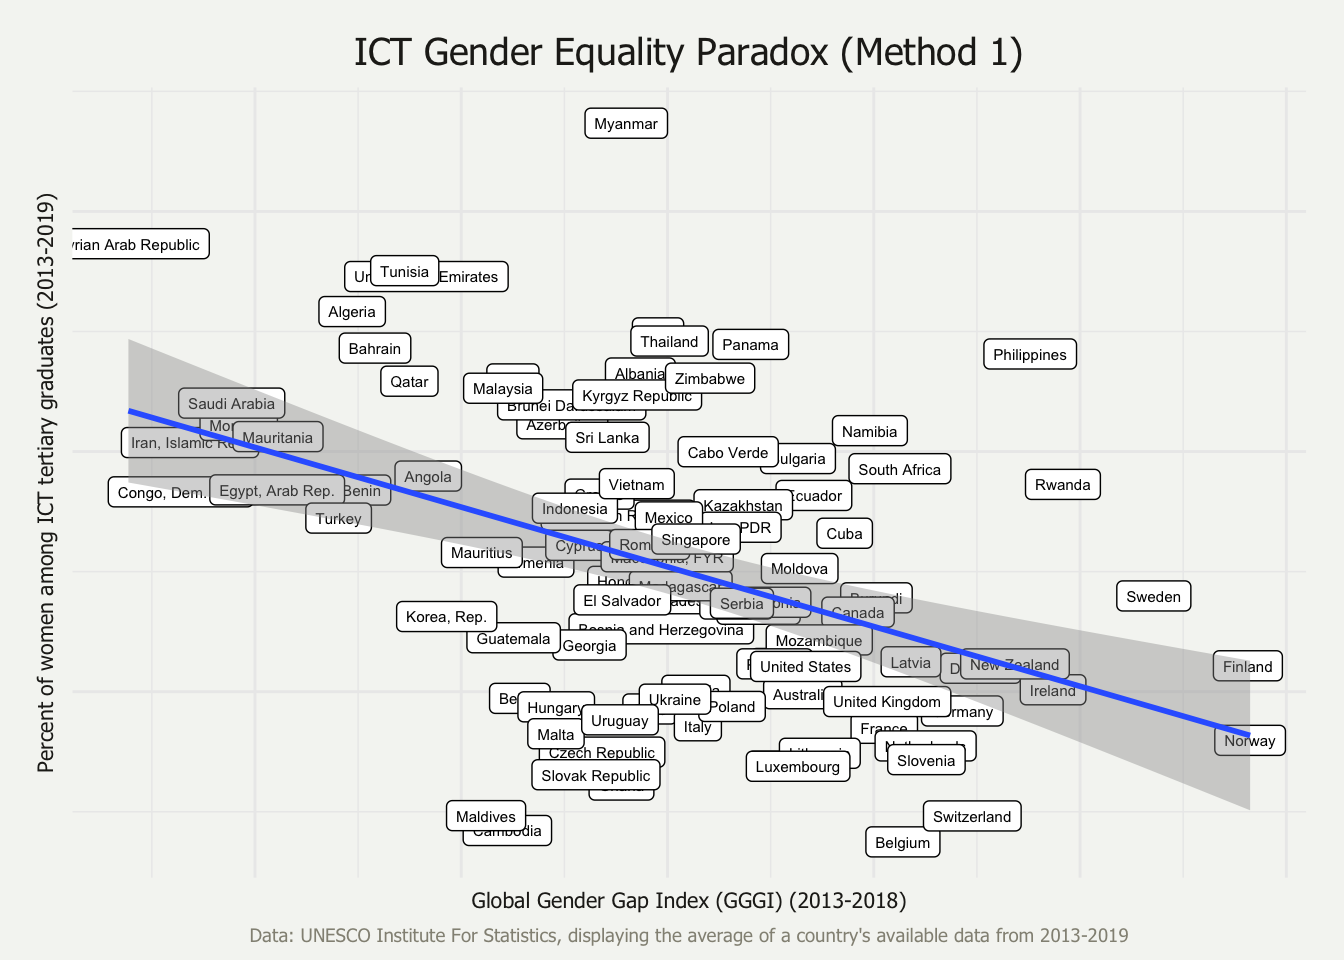
\includegraphics{bookdown-demo_files/figure-latex/ict_cor_1-1.pdf}

\section{The ICT-GEP after adjusting the percentages to reflect when
equal numbers of men and women graduate with tertiary degrees within
each
country}\label{the-ict-gep-after-adjusting-the-percentages-to-reflect-when-equal-numbers-of-men-and-women-graduate-with-tertiary-degrees-within-each-country}

This method replicates Stoet \& Geary's (2018) \emph{propensity} method,
where they estimate the percentage of women among STEM graduates when
there are an equal number of men and women graduates overall. In this
case, in the formula \(a/(a + b)\), \(a\) represents the percentage of
women graduates who graduate from an ICT program, and \(b\) represents
the percentage of men graduates who graduate from an ICT program. Stoet
\& Geary (2018) explain that they use Spearman's correlation coefficient
because some of the variables are not normally distributed. However, the
variables are continuous, and it is a misconception that variables must
be normally distributed in order to use the more robust Pearson's
correlation coefficient \citep{nefzgerNeedlessAssumptionNormality1957}.
Following the \emph{propensity} method, but using the Pearson test, GGGI
is moderately, negatively correlated with the estimated percentage of
women among ICT assuming equal graduation numbers of men and women
(\emph{r} = -0.47, \emph{p} \textless{} 0.001). For the sake of
comparison (though not endorsed), the \emph{propensity} method paired
with Spearman's test also results in a moderate, negative correlation
(\(\rho\) = -0.40, \emph{p} \textless{} 0.001) to a lesser extent.

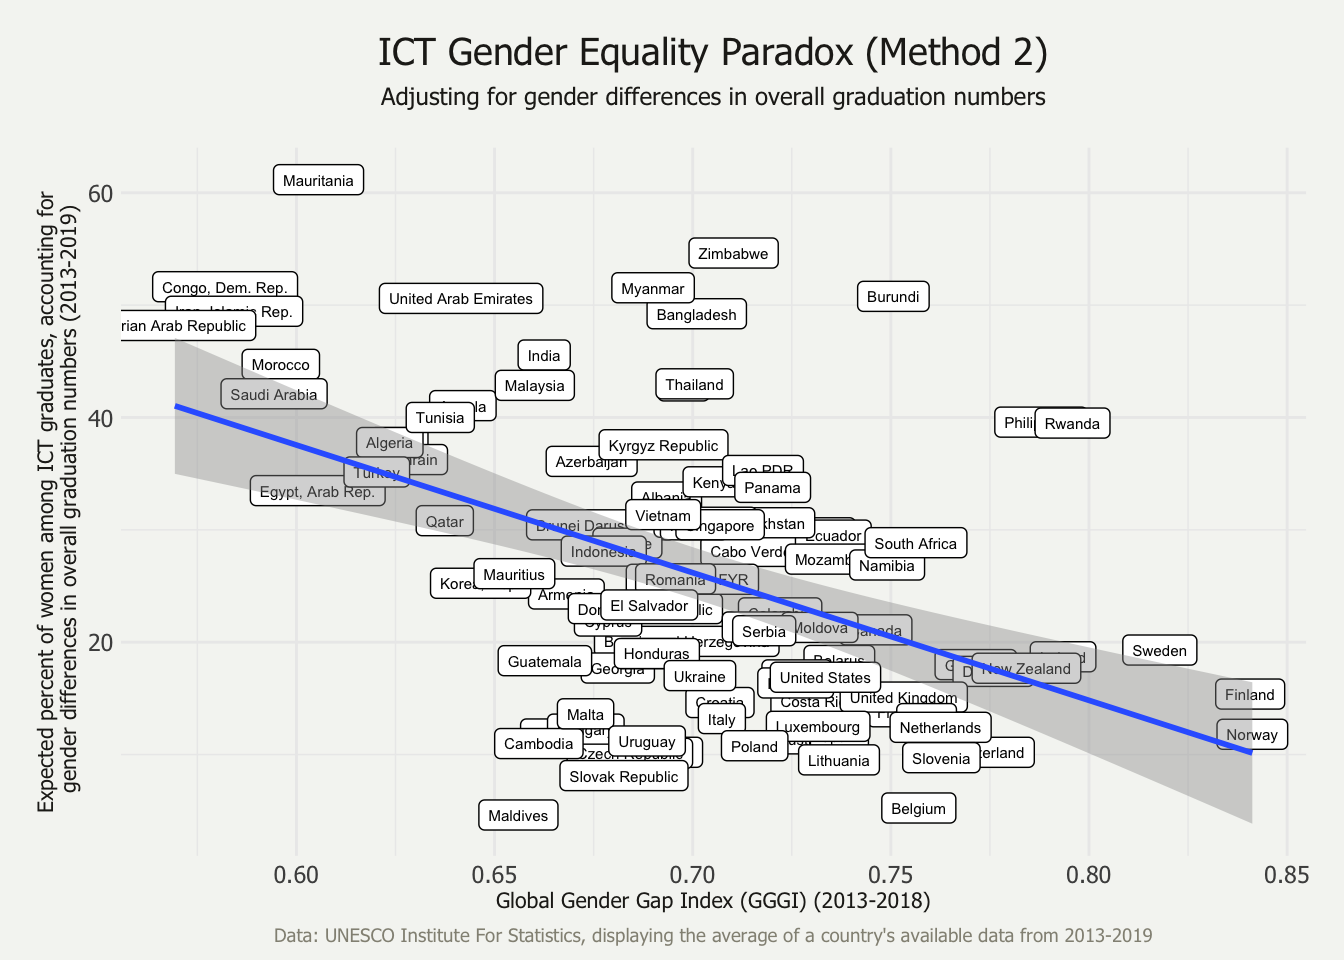
\includegraphics{bookdown-demo_files/figure-latex/ict_cor_2-1.pdf}

\section{The ICT-GEP as a function of the disparity between ICT
graduation rates for men and
women}\label{the-ict-gep-as-a-function-of-the-disparity-between-ict-graduation-rates-for-men-and-women}

The final method is unique from the methods utilized or posed by Stoet
\& Geary, Richardson et al., and UNESCO. This \emph{disparity} method
considers the correlation between the GGGI and the disparity between the
percent of women graduates and percent of men graduates who graduate
from an ICT program. There is a weak correlation between GGGI and this
disparity index (\emph{r} = -0.30, \emph{p} \textless{} 0.01).

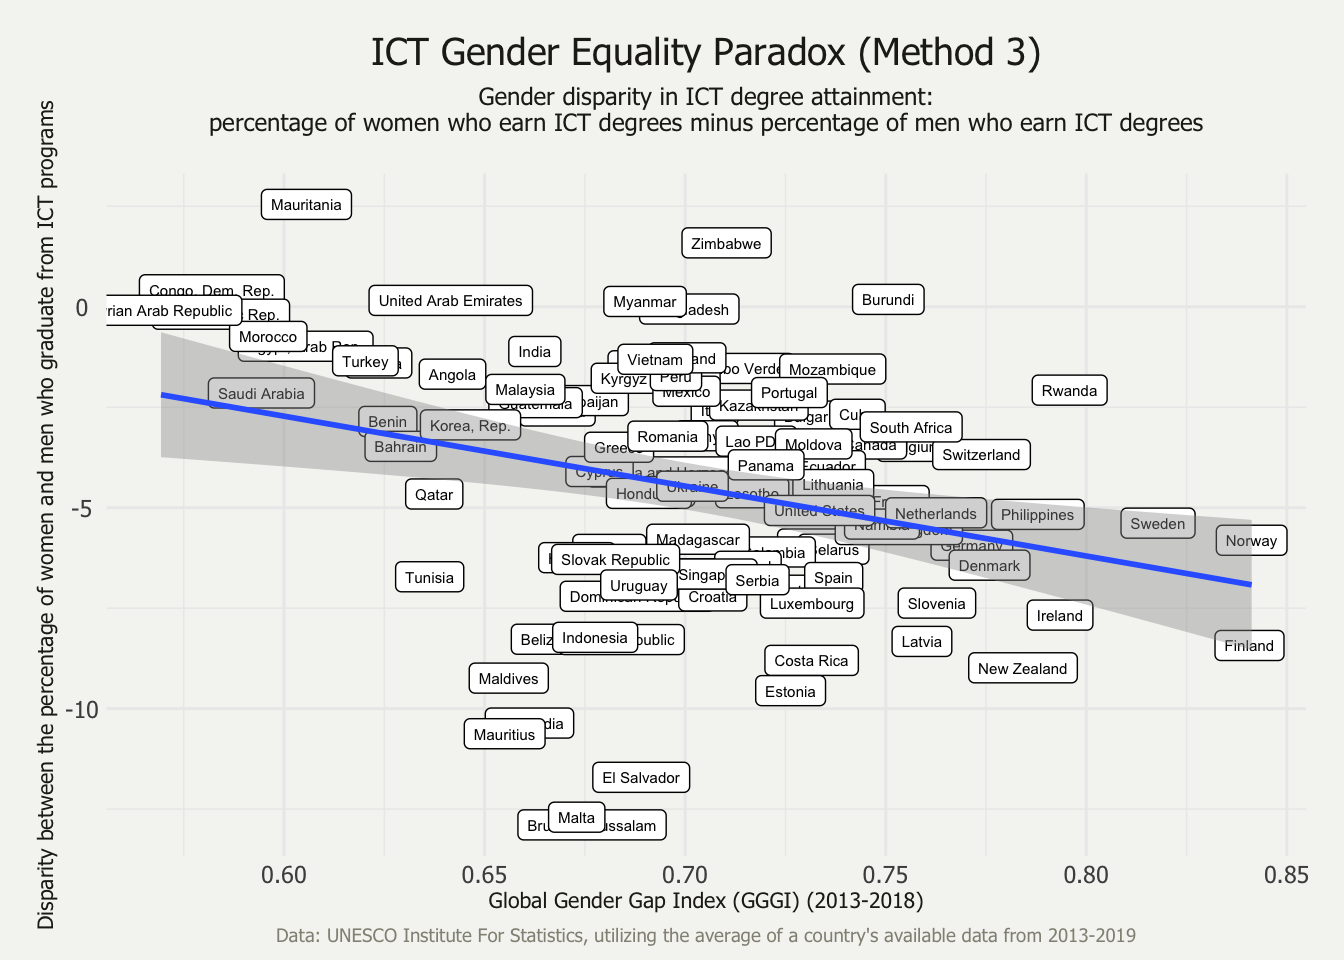
\includegraphics{bookdown-demo_files/figure-latex/ict_cor_3-1.pdf}

\section{Correlation comparison}\label{correlation-comparison}

Are the three correlation methods equivalent to each other? One method
may have more theoretical support for its usage, but this step of the
analysis concerns whether that methodological decision bears any impact
of the conclusions of the analysis. The three correlations compose a set
of dependent, overlapping correlations. That is, the correlations are
dependent on each other because all three share a common variable, the
GGGI. The \texttt{cocor()} function from the \texttt{cocor} package
\citep{diedenhofenCocorComprehensiveSolution2015} was used with the
formula for dependent, overlapping correlations to test for a
significant difference between each pair of the correlations. Ten
different tests\footnote{The ten tests for correlation comparison are
  Pearson and Filon's z (1898), Hotelling's t (1940), Williams' t
  (1959), Olkin's z (1967), Dunn and Clark's z (1969), Hendrickson,
  Stanley, and Hills' (1970) modification of Williams' t (1959),
  Steiger's (1980) modification of Dunn and Clark's z (1969) using
  average correlations, Meng, Rosenthal, and Rubin's z (1992), Hittner,
  May, and Silver's (2003) modification of Dunn and Clark's z (1969)
  using a backtransformed average Fisher's (1921) Z procedure, and Zou's
  (2007) confidence interval} were run for each comparison; the results
of the three comparisons reflects unanimous results from the ten tests.
Results of Steiger's (1980) test are reported.

The correlation results from Method \#1 and Method \#2 are equivalent
(\emph{z} = 0.9674, \emph{p} = 0.33), thus, using either the raw
percentage of women among ICT graduates or the expected percentage
adjusted for the gender disparity in overall graduation results in
statistically equivalent correlations with the GGGI.

The correlation results from Method \#1 and Method \#3 are also
equivalent (\emph{z} = -1.32, \emph{p} = 0.19), thus using either the
raw percentage of women among ICT graduates or the disparity between the
percentage of women versus men graduates who graduate from ICT programs
results in statistically equivalent correlations with the GGGI.

Lastly, the correlation results from Method \#2 and Method \#3 are not
equivalent (\emph{z} = -2.30, \emph{p} \textless{} 0.05). Though Methods
\#2 and \#3 do not produce equivalent correlations, the two methods
debated by Stoet \& Geary (2020) and Richardson et al. (2020) do produce
equivalent correlations. Similarly, Stoet \& Geary (2020) re-analyzed
the STEM-GEP using Method \#1, which also resulted in a statistically
significant, moderate, and negative correlation. However, Stoet \& Geary
(2020) did not statistically test for the equivalence of the two
correlations, which could have strengthened their argument.

\chapter{Discussion}\label{discussion}

The ICT-GEP as presented in the UNESCO report on digital skills and
gender lacks many of the statistical details expected in research
reports of this nature. Many unknowns about the exact methods employed
remain, including, but not limited to: selection criteria, consideration
of outliers, and tests used to measure correlation. This re-analysis
confirmed that there is a moderate, negative correlation between GGGI
and the percent of women among ICT graduates. Additionally, this
correlation is equivalent to the correlation produced when adjusting for
the disparity between the base number of women and men graduates. A
third correlation concerning the disparity between the percentage of
women and men graduates who graduate from an ICT program produced a
weaker correlation that is not equivalent to the other two correlation
methods.

These findings demonstrate the need for further scrutinization of the
methods employed by Stoet \& Geary (2018) and the UNESCO Thinkpiece.
Further consensus and clarification is needed before countries accept
these results as evidence for the necessity (or lack thereof) of
particular policy interventions.

Future research should further investigate the validity of using the
GGGI as the index of gender equality and consider alternatives other
than the BIGI. Other variables besides gender equality should also be
examined, such as the size of the ICT industry in each country. Future
qualitative research should also be considered to avoid some of the
pitfalls of this quantitative approach, like the possibility of spurious
correlation. For example, interviews of women who pursued an
undergraduate ICT education in an Arab State but a graduate ICT
education in a European country would offer a wealth of information
about the potential factors underlying the ICT-GEP hypothesis.

\section{tldr;}\label{tldr}

A 2019 UNESCO report \citep{westBlushIfCould2019a} dedicated a think
piece to the ICT Gender Equality-Paradox, displaying a paradoxical
correlation--- the higher the gender equality in a country, the lower
the percentage of women among ICT (computer science and related
subjects) graduates. The broader STEM gender-equality paradox has been
challenged \citep{richardsonThereGenderEqualityParadox2020a} for
methodological reasons, but the ICT gender-equality paradox has yet to
receive similar scrutiny despite its almost parallel methods. Thus, the
present analysis took a deeper look into the ICT Gender-Equality
Paradox, uncovering the following:

\begin{itemize}
\tightlist
\item
  The UNESCO report does not provide transparency of any kind in regards
  to this finding (e.g., the think piece does not provide information on
  data cleaning/omission, descriptive or even inferential statistics).
  The only evidence to support their finding is a visual representation
  of the paradox in graph form.
\item
  The two different, contested methods for performing the correlation
  test (see \citet{richardsonThereGenderEqualityParadox2020a} \&
  \citet{stoetGenderEqualityParadoxPart2020a}) result in statistically
  equivalent correlations (informed by a suite of ten tests meant to
  test for the equality of correlations, not just the presence of two
  statistically significant correlation results as reported by
  \citet{stoetGenderEqualityParadoxPart2020a}. Thus, equal correlations
  result whether or not women and men's graduation base rate is taken
  into account.
\item
  A third correlation approach utilizing the disparity between the
  percentage of all women versus all men graduates who graduate from an
  ICT program is not equivalent to the aforementioned correlations,
  though a significant (though weaker) correlation does result.
\end{itemize}

Overall, this re-analysis points to multiple, specific weaknesses in
UNESCO's reporting of an ICT Gender-Equality Paradox. In addition to
these weaknesses, it remains possible that the relationship between
gender equality and ICT graduation gender patterns is a spurious
correlation. Further research should, therefore, be required before the
ICT Gender-Equality Paradox is accepted as anything beyond a hypothesis
or thought experiment.

\bibliography{ict-gep.bib}

\end{document}
